%\addcontentsline{toc}{chapter}{Development Process}
\chapter{Design}

You should concentrate on the more important aspects of the design. It is essential that an overview is presented before going into detail. As well as describing the design adopted it must also explain what other designs were considered and why they were rejected.

The design should describe what you expected to do, and might also explain areas that you had to revise after some investigation.

Typically, for an object-oriented design, the discussion will focus on the choice of objects and classes and the allocation of methods to classes. The use made of reusable components should be described and their source referenced. Particularly important decisions concerning data structures usually affect the architecture of a system and so should be described here.

How much material you include on detailed design and implementation will depend very much on the nature of the project. It should not be padded out. Think about the significant aspects of your system. For example, describe the design of the user interface if it is a critical aspect of your system, or provide detail about methods and data structures that are not trivial. Do not spend time on long lists of trivial items and repetitive descriptions. If in doubt about what is appropriate, speak to your supervisor.
 
You should also identify any support tools that you used. You should discuss your choice of implementation tools - programming language, compilers, database management system, program development environment, etc.

Some example sub-sections may be as follows, but the specific sections are for you to define. 

\begin{figure}
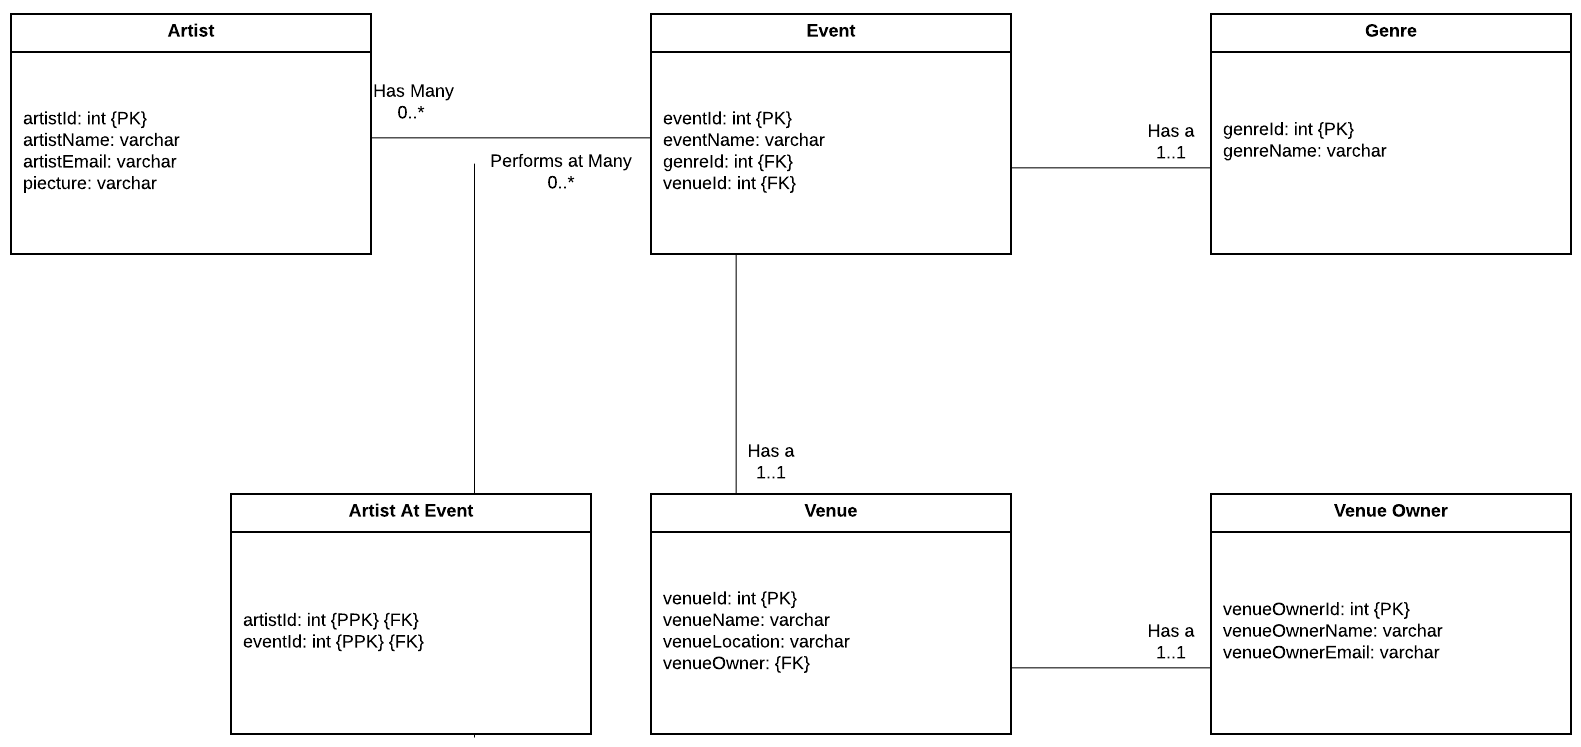
\includegraphics[width=\textwidth,height=\textheight,keepaspectratio]{images/events}
\caption{UML diagram which illustrates the appropriate relationships between the different tables in the database in relation to an event. Crested using https://www.lucidchart.com/}
\end{figure}

\section{Overall Architecture}

\section{Some detailed design}

\subsection{Even more detail}

\section{User Interface}

\section{Other relevant sections}